% file: 3-9-connectivity/2conn-cut-vertex.tex

\documentclass[tikz]{standalone}
\usetikzlibrary{positioning, decorations.pathmorphing, fit, shapes}

\begin{document}
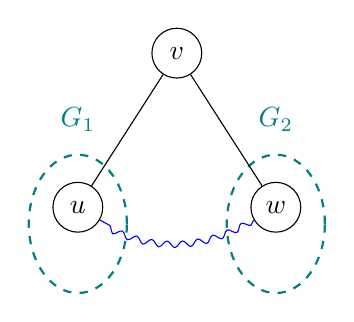
\begin{tikzpicture}[every node/.style = {draw, circle, minimum size = 18pt},
    node distance = 1.5cm and 0.8cm,
    path/.style = {-, decorate, decoration = {snake, amplitude = .4mm, segment length = 2mm, post length = 1mm}},
    comp/.style = {yshift = -6pt, draw, thick, dashed, teal, ellipse, minimum height = 50pt, minimum width = 18pt}]
  \node (v) {$v$};
  \node (u) [below left = of v] {$u$};
  \node (w) [below right = of v] {$w$};

  \node [fit = (u), comp, label = {[above, teal] $G_1$}] {};
  \node [fit = (w), comp, label = {[above, teal] $G_2$}] {};

  \path (v) edge (u)
  	    edge (w)
	(w) edge[blue, bend left, path] (u);
\end{tikzpicture}
\end{document}
